\ifx\PREAMBLE\undefined
\documentclass[fleqn]{article}
\usepackage{geometry}
\usepackage[format = hang, font = bf]{caption}
\usepackage{subcaption}
% The following is needed in order to make the code compatible
% with both latex/dvips and pdflatex. Added for using UML generated by MetaUML.
\ifx\pdftexversion\undefined
\usepackage[dvips]{graphicx}
\else
\usepackage[pdftex]{graphicx}
\DeclareGraphicsRule{*}{mps}{*}{}
\fi
\usepackage{array}
\newcolumntype{C}[1]{>{\centering\let\newline\\\arraybackslash}b{#1}}
\newcommand{\parcell}[2][l]{\begin{tabular}{@{}#1@{}}#2\end{tabular}}
\usepackage{pdflscape}
\usepackage{multirow}
\usepackage{graphicx}
\usepackage{floatrow}
\floatsetup[table]{capposition=top}
\usepackage{bigstrut}
\usepackage{supertabular}
\usepackage{booktabs}
\usepackage{amsmath}
\usepackage{listings}
\usepackage{multicol}
\usepackage{xcolor}
\usepackage{mathrsfs}%mathcal
\usepackage{amsfonts}%allowing \mathbb{R}
\usepackage{amssymb}
\usepackage{alltt}
\usepackage{xspace}
\usepackage{color}
\usepackage{wrapfig}%text around figure
\usepackage{lipsum}
\usepackage{tikz}
\usetikzlibrary{shapes,positioning}
\usepackage{url}
\def\UrlBreaks{\do\A\do\B\do\C\do\D\do\E\do\F\do\G\do\H\do\I\do\J\do\K\do\L\do\M\do\N\do\O\do\P\do\Q\do\R\do\S\do\T\do\U\do\V\do\W\do\X\do\Y\do\Z\do\[\do\\\do\]\do\^\do\_\do\`\do\a\do\b\do\c\do\d\do\e\do\f\do\g\do\h\do\i\do\j\do\k\do\l\do\m\do\n\do\o\do\p\do\q\do\r\do\s\do\t\do\u\do\v\do\w\do\x\do\y\do\z\do\0\do\1\do\2\do\3\do\4\do\5\do\6\do\7\do\8\do\9\do\.\do\@\do\\\do\/\do\!\do\_\do\|\do\;\do\>\do\]\do\)\do\,\do\?\do\'\do+\do\=\do\#\do\-}
\usepackage{xr}%allow cross-file references
\usepackage[breaklinks = true]{hyperref}
\lstset{
language = C, 
showspaces = false,
breaklines = true, 
tabsize = 2, 
extendedchars = false, 
basicstyle = {\ttfamily \footnotesize}, 
showstringspaces=false,
keywordstyle=\color{blue!70}, 
commentstyle=\color{gray},
rulesepcolor=\color{red!20!green!20!blue!20}, 
numberstyle=\color[RGB]{0,192,192},
stringstyle=\color{red},
escapeinside={ )},
moredelim=[is][\underbar]{(**}{**)},
mathescape
}
\mathchardef\myhyphen="2D
\begin{document}
\fi
\newpage
\section{Virtual Memory}
Virtual memory provides 3 important abilities:
\begin{enumerate}
	\item It uses the main memory efficiently by treating a cache for a namespace stored on the disk.
	\item It simplifies memory management by providing each process with a uniform address space.
	\item It protects the address space of each process from being corrupted by other processes.
\end{enumerate}
\subsection{Introduction}
\subsubsection{Virtual address space}
The main memory is organized as a M-byte consecutive array. Each byte has a unique \textbf{physical address} starting from 0. CPU can access memory with its physical address, namely \textbf{physical addressing}. Modern processors use \textbf{virtual addressing} to access memory. CPU generates a \textbf{virtual address} to access memory. The VA is translated into a physical address by the \textbf{memory management unit(MMU)} on the CPU chip before being sent to the main memory. CPU generates VA inside a \textbf{virtual address space} $\{0, 1, 2, \dots, N-1\}$ with $N=2^n$. Similarly there is a \textbf{physical address space} $\{0,1,2,\dots,M-1\}$. We assume $M=2^m$.
\subsubsection{VM as cache}
Conceptionally, VM is organized as a N-byte consecutive array on the disk. Each byte has a unique VA. Data on the disk is cached inside the main memory. Like other caches in the memory hierarchy, data on the disk is divided into blocks to serve as basic units for transportation between the disk and the main memory. The virtual memory is divided into \textbf{virtual pages(VP)} of size $P=2^p$, and the physical memory is divided into \textbf{physical pages(PP)}, or \textbf{page frames} of the same size. At any time, the set of VPs is divided into 3 subsets: 
\begin{itemize}
	\item Unallocated: pages not yet created by the VM system. Not related to any data, thus occupies no disk space.
	\item Cached: Allocated and cached in the physical memory.
	\item Uncached: Allocated but not cached in the memory.
\end{itemize}
Cost of DRAM cache miss is enormous:
\begin{itemize}
	\item DRAM 10 times slower than SRAM; hard disk 100000 times slower than DRAM.
	\item Cost of reading the first byte from a disk sector is 100000 times higher than that of reading further bytes consecutively.
\end{itemize}
Properties of DRAM cache: large pages (4KB-2MB); full associative (any VP can be put in any PP); write-back instead of write-through.

\textbf{Page table} is used to tell if a VP is cached inside a PP; if so, which PP; if not, where is it on disk. It's an array of PTE(page table entry)s stored in memory and managed by the OS. Each VP is related to a PTE in the page table. A PTE has a valid bit and an n-bit address segment, which is used to indicate the starting address of the PP in DRAM if the valid bit is set (1), or the starting address of the PP on disk if the valid bit is unset (0). If the VP is unallocated, the valid bit is 0 and the address is set to null. 

A DRAM cache miss is called a page fault. An exception handler in the kernel will be called. The needed VP will be copied into a PP at the cost of a sacrificed page. The instruction that caused the page fault will be executed again.

The efficiency of VM is guaranteed by locality. Programs tend to work mainly on a small set of pages called the working set. After some initial cost, page fault is supposed to be rare.
\subsubsection{VM as tool for memory management}
\begin{itemize}
	\item VM simplifies linking. A separate virtual address space allows each process to use the same basic format for its memory image, e.g. \texttt{.data} always starts at 0x400000. The implementation of the linker is greatly simplified.
	\item VM simplifies loading. Loader does not have to copy any data from disk to memory. All it does is to allocate VPs for \texttt{.text} and \texttt{.data} segments of the executable and mark them as uncached. They will be paged in by the VM automatically on demand.
	\item VM simplifies data \& code sharing. Different processes can share data \& code, e.g. C standard libraries and kernel codes, by mapping VPs in their virtual address spaces to the same PPs.
	\item VM simplifies memory allocation. Consecutive VPs do not have to be mapped to consecutive PPs.
\end{itemize}
\subsubsection{VM as tool for memory protection}
\begin{itemize}
\item Separate virtual address space makes it easy to isolate private memories of different processes. 
\item Additional control bits can be added to PTEs for memory protection. For example, a SUP bit can be used to restrict access of the VP to super user; READ/WRITE bits can be used to allow and forbid processes from reading and writing the VP. If such restrictions are violated, the CPU triggers a protection fault, which is reported as ``segmentation fault'' in Linux.
\end{itemize}
\subsection{Memory Translation}
Memory translation is a map from the virtual address space to the physical address space:
\begin{gather*}
MAP:VAS\rightarrow PAS\cup\emptyset\\
MAP(A)=\begin{cases}
A'&\text{If data at VA A is at PA A'}\\
\emptyset&\text{If data at VA A is not in physical memory}
\end{cases}
\end{gather*}
\begin{description}
	\item[PTBR]Page table base register: a control register in the CPU. Points to the current page table.
	\item[VPN]Virtual page number.
	\item[VPO]Virtual page offset in bytes. Last p bits of VA.
	\item[PPN]Physical page number.
	\item[PPO]Physical page offset in bytes. Last p bits of PA. Equal to VPO.
\end{description}
Page hit:
\begin{enumerate}
	\item CPU generates a VA and sends it to the MMU.
	\item MMU generates the address of the appropriate PTE (PTBR + VPN), and asks SRAM/DRAM for the PTE.
	\item SRAM/DRAM returns the PTE to the MMU.
	\item MMU obtains the PPN from the PTE, and constructs the PP(PPN + VPN). The PP is sent to SRAM/DRAM.
	\item SRAM/DRAM returns the asked word to the CPU.
\end{enumerate}
Page fault:
\begin{enumerate}
	\item 1-3: the same as page hit.
	\item The valid bit of the PTE is 0. MMU triggers an exception. Control is transferred to the page fault exception handler in the kernel.
	\item The handler identifies a victim page in the physical memory. If it has been modified, it's paged out to the disk.
	\item The handler pages in the new page (whose address on disk is in the PTE) and updates the PTE.
	\item The handler returns control to the original process and the instruction is executed again.
\end{enumerate}
\begin{description}
\item[TLB]Translation lookaside buffer. A small buffer in the MMU dedicated to PTEs. It's usually highly associative. If TLB has $2^t$ sets, then the least significant t bits of the VPN is used as the TLBI(TLB index) and the rest is used as TLBT(TLB tag).
\item[Multi-level Page Tables]One single page table calls for too much memory footprint. With a 32-bit address space, 4KB pages and 4B PTEs, a 4MB page table has to stay in memory. For a 64-bit address space it's even large. The page table can be compacted with a hierarchy of page tables. 
\begin{figure}[ht]
\centering
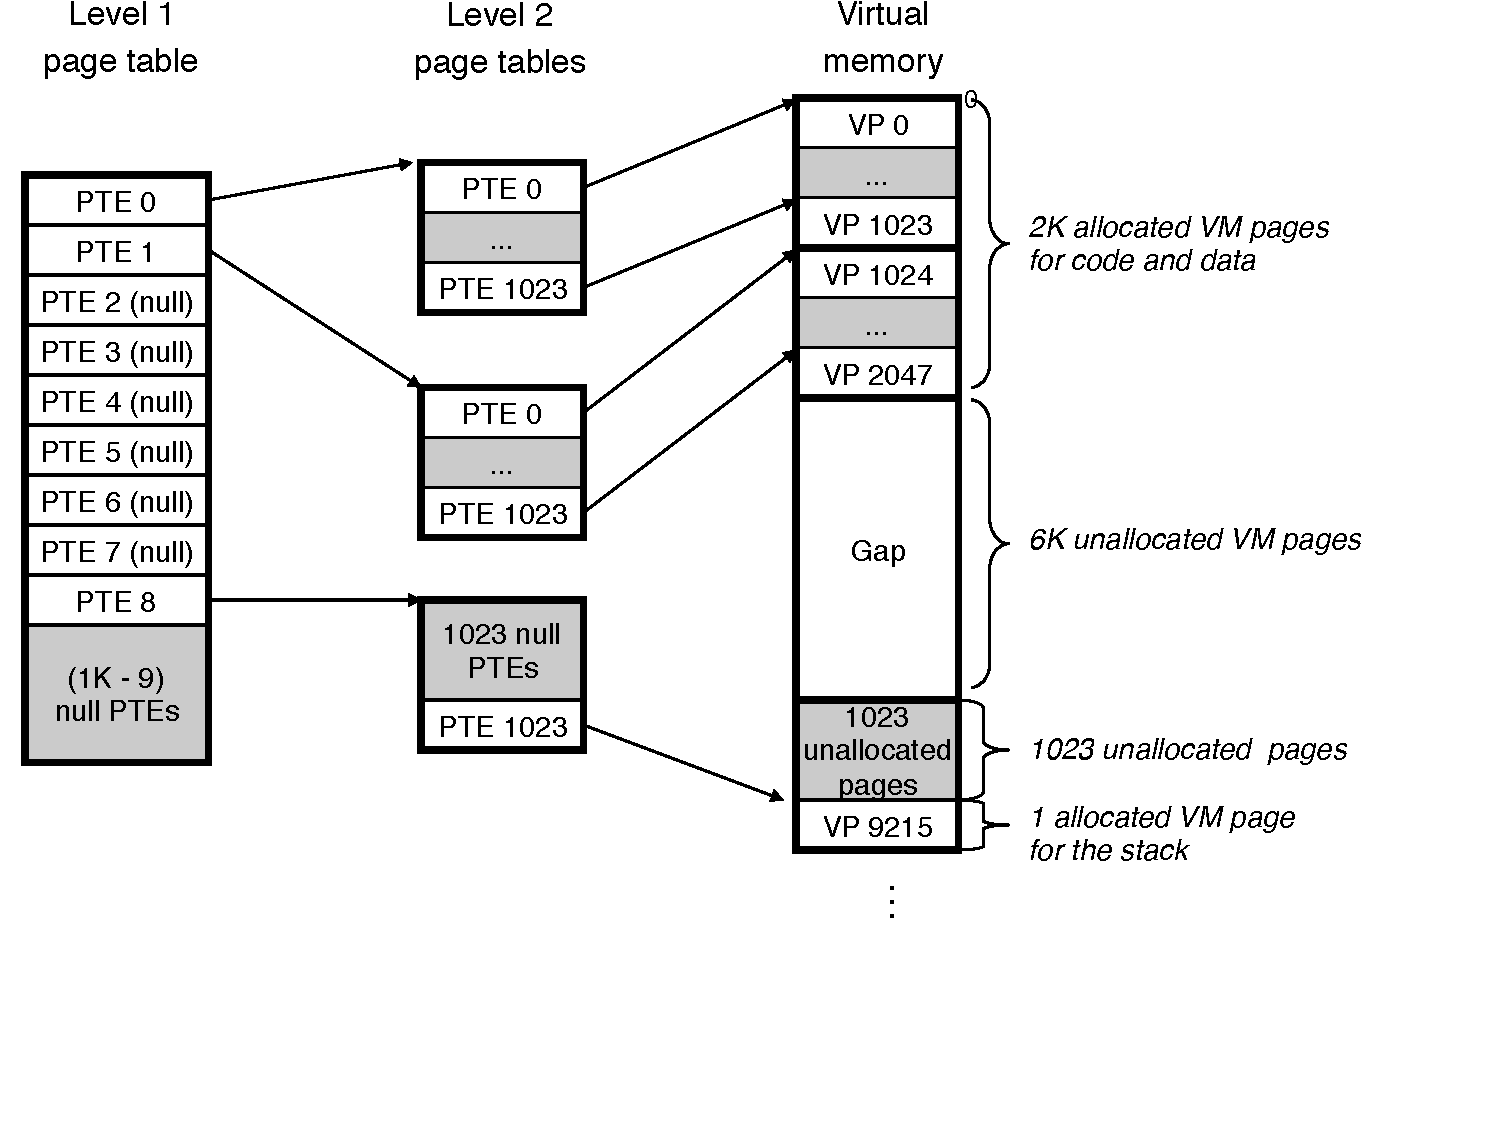
\includegraphics[width=0.8\textwidth]{multilevel.pdf}
\caption{A 2-level page table hierarchy}
\end{figure}

As shown in the figure, each entry in the 1st level page table is responsible for a 4MB chunk in the VAP, which is 1024 VPs. If none of the pages in the chunk is allocated, the entry in the 1st level page table is empty. If at least one of them is allocated, the entry points to the address of a 2nd level page table.
\end{description}
\subsection{Case study: Intel Core i7/Linux VM system}
\subsubsection{Intel Core i7 memory translation}
\begin{itemize}
\item Core i7 uses 48-bit VAS (256TB) and 52-bit PAS (4PB). 
\item L1 d-cache: 32KB, 64B block, 8-way associative, thus 64 sets. PA: 40-bit CT, 6-bit CI, 6-bit CO.
\item 4-level page table. VA: 4$\times$ 9-bit VPNs + 12-bit VPO. Level 1: 512GB each entry. Level 2: 1GB. Level 3: 2MB. Level 4: 4KB (page size).
\item Parallel address translation: 12-bit VPO = 12-bit PPO = 6-bit CI + 6-bit CO, thus PPN = CT. During address translation, VPN is transferred to MMU while VPO is transferred to L1 d-cache. When MMU asks TLB for a PTE, L1-cache finds the appropriate set according to CI and reads the 8 tags and data words (according to CO). After the MMU obtains PPN from TLB, it simply compares it against the 8 tags and choose the word whose tag matches (in case of a cache hit).
\end{itemize}
\subsubsection{Linux VM system}
Linux maintains a separate VM space for each process. VM is organized as a collection of areas(segments). An area is a contiguous chunk of existing (allocated) VM whose pages are related in some way. Each existing VP is contained in an area. Any VP that is not part of some area does not exist, cannot be referenced by the process, and does not consume any additional resources.
\begin{wrapfigure}{R}{0.5\textwidth}
\centering
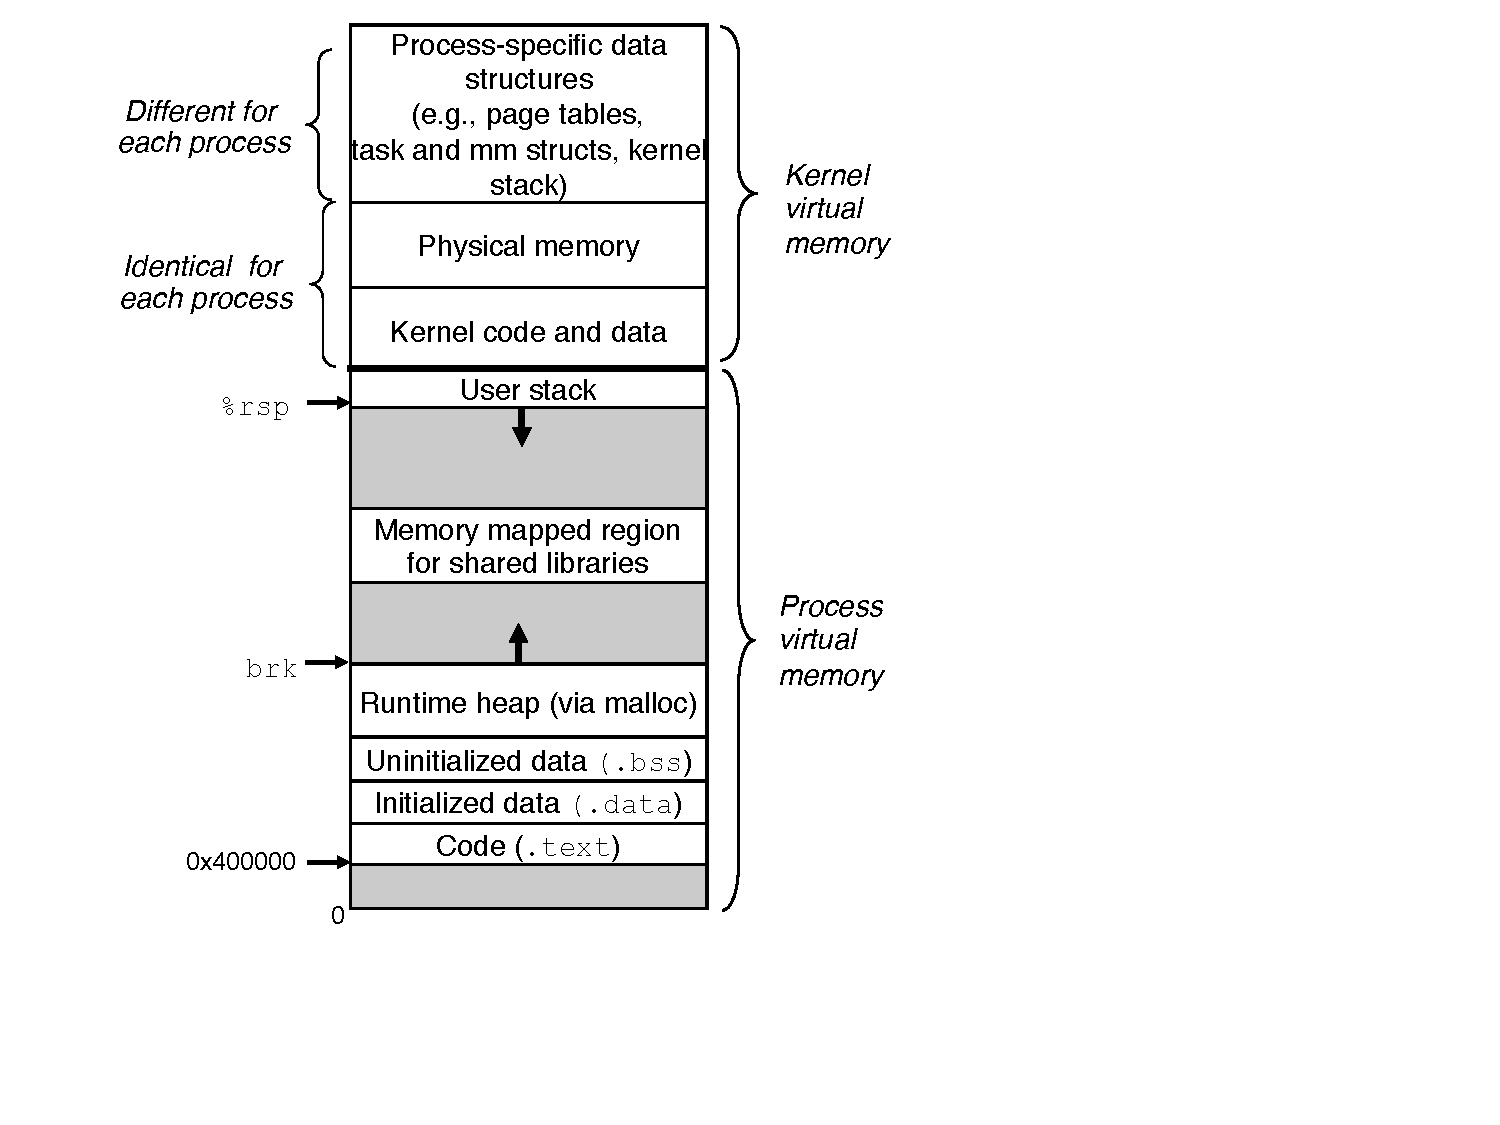
\includegraphics[width=\textwidth]{processimage.pdf}
\caption{VM of a Linux process}
\end{wrapfigure}

Kernel data structures used to keep track of VM areas of a process:
\begin{itemize}
\item A separate task struct for each process (\texttt{task\_struct}). Its elements either contain of point to information needed by the kernel to run the process: PID, pointer to the user stack, name of the executable file, PC, etc.
\item One of the entries points to an \texttt{mm\_struct} that characterizes the current state of the VM. It contains:
\begin{itemize}
	\item \texttt{pgd}: base of the level 1 page table.
	\item \texttt{mmap}: a list of \texttt{vm\_area\_structs}, each of which characterizes an area. 
\end{itemize}
\item \texttt{vm\_area\_structs} contains:
\begin{itemize}
	\item \texttt{vm\_start}: points to the beginning of the area.
	\item \texttt{vm\_end}: points to the end of the area.
	\item \texttt{vm\_prot}: read/write permissions for all pages in the area.
	\item \texttt{vm\_flags}: whether pages in the area are shared with other processes, etc.
	\item \texttt{vm\_next}: points to the next area struct in the list.
\end{itemize}
\end{itemize}

Linux page fault exception handling:
\begin{enumerate}
\item Check if the VA is legal, i.e. if the VA is contained in an area, by comparing it against \texttt{vm\_start} and \texttt{vm\_end} in each area struct. If illegal: segmentation fault.
\item Check if the access is legal, i.e. if the process has enough permissions to read/write/execute the pages in the area. If illegal: protection exception.
\item Page out victim page and page in the new page. Re-execute the instruction.
\end{enumerate}
\subsection{Memory mapping}	
Linux \textbf{initializes}\footnote{Further changes made to VM areas are not necessarily reflected back to the original objects on disk. See below (private areas).} the contents of a VM area by associating it with an object on disk. The process is called memory mapping. Areas can be mapped to two kinds of objects: 
\begin{itemize}
	\item Regular. A contiguous section of a regular disk file. The section is divided into page-size pieces, each containing the initial contents of a VP. Because of demand paging, no VP is actually swapped into physical memory until the page is touched by the CPU.
	\item Anonymous. An anonymous file created by the kernel containing only binary zeros. When the page is first touched, a victim page in the physical memory is overwritten with 0. No data is transferred between disk and memory.  
\end{itemize}
Once a VP gets initialized, it is swapped back and forth between the physical memory and the swap file on disk\footnote{Looks like an error in the book. ``Swapped between a swap file''?}. The size of the swap file bounds the number of VPs that can be allocated by the running processes. 

Let's revisit some concepts introduced before.
\begin{description}
\item[Shared Object]An object can be mapped to an area of VM as either a shared object or a private object. Any writes made by an process to the area in its VM mapped to a shared object are visible to other processes that also map the shared object into their VMs, and are reflected in the original object on disk. On the contrary, changes made to an area mapped to an private object are not visible to other processes. Neither are they reflected back to the object on disk. 

Private objects are mapped into VM using copy-on-write technique. Multiple processes can map the same private object on disk into their VMs. Related PTEs are flagged as read-only, and related area structs are flagged as \textbf{private copy-on-write}. Only a single copy of the private object is kept in the physical memory until either process attempts to write to some page in the private area, when a protection fault is triggered. A new copy of the page will be created in the memory, with the related PTE updated. The process will have write permission to the new page.
\item[fork]When the current process calls the \texttt{fork} function, the kernel creates various data structures for the new process and assigns it a unique PID. In order to create VM for the new process, it create exact copies of the current process's \texttt{mm\_struct}, area structs and page table. All pages in both processes are flagged as read-only, and all area structs are flagged as private copy-on-write. When either process performs writes, new pages will be created by the copy-on-write mechanism. The abstraction of a private address space for each process is preserved.
\item[execve]\texttt{execve("a.out", NULL, NULL);} loads and runs the program contained in the executable object file \texttt{a.out} within the current process, effectively replacing the current program with the \texttt{a.out} program. This is accomplished in the following steps:
\begin{itemize}
	\item Delete existing area structs in the user portion of the current process's VM.\footnote{Maybe also the page table?}
	\item Map private areas. New area structs are created for the code, data, bss, stack and heap areas of the new programs, all of whom are private copy-on-write. Code and data areas are mapped to \texttt{.text} and \texttt{.data} sections of \texttt{a.out}. Bss is mapped to an anonymous file whose length is contained in \texttt{"a.out"}. Stack and heap are mapped to an anonymous file of initial length 0. 
	\item Map shared areas. Shared objects such as \texttt{libc.so} are mapped into the shared region of the VM.
	\item Set the PC of the current process's context to the entry point in the code area. 
\end{itemize}
\end{description}

Linux processes can use the \texttt{mmap} function to create new VM areas and map objects to these areas. 
\begin{lstlisting}[frame=single]
#include <unistd.h>
#include <sys/mman.h>
void *mmap(void *start, size_t length, int prot, int flags, int fd, off_t offset);
int munmap(void* start, size_t length);
\end{lstlisting}
\texttt{mmap} asks the kernel to create a new VM area mapped to a contiguous chunk of the object specified by file descriptor \texttt{fd}. The size of the chunk is \texttt{length} and it starts from \texttt{offset} bytes from the beginning of the file. \texttt{start} is the suggested beginning address of the new area, usually specified as NULL. \texttt{prot} contains access permissions of the new area (i.e. \texttt{vm\_prot} in its area struct). It can be 
\begin{itemize}
	\item PROT\_EXEC: pages within the area are composed of instructions executable by the CPU. 
	\item PROT\_READ: pages within the area are readable.
	\item PROT\_WRITE: pages within the area are writeable.
	\item PROT\_NONE: pages within the area cannot be accessed. 
\end{itemize}
\texttt{flags} describes type of the object. They can be ORed with $|$.
\begin{itemize}
	\item MAP\_ANON: anonymous object.
	\item MAP\_PRIVATE: private copy-on-write.
	\item MAP\_SHARED: shared object. 
\end{itemize}
\texttt{munmap} deletes an area created by \texttt{mmap}.
\subsection{Dynamic memory allocation}
Dynamic memory allocation is necessary because we often do not know the size of some data structures until runtime. 
\subsubsection{Requirements}
\begin{itemize}
	\item Handle arbitrary sequence of requests. No assumption should be made about the sequence of allocate / free requests except that each free request should correspond to a previous successful allocate request.
	\item Reply to requests immediately. The allocator is not allowed to reorder or buffer requests to improve efficiency.
	\item Use only the heap.
	\item Align the blocks so that any data object can be stored.
	\item Leave allocated blocks unmodified. The allocator can only manipulate or change free blocks.
\end{itemize}
\subsubsection{Performance goals}
\begin{itemize}
	\item Maximize throughput, i.e. requests handled per minute. Reasonable performance: the worst running time of an allocate request is linear in the number of free blocks, while the free request can be finished in constant time.
	\item Maximize memory utilization. Peak utilization:
	$$U_k=\frac{\max_{i\le k}P_i}{\max_{i\le k}H_k}.$$
	$P_k$ is the aggregate payload after request $R_k$ and $H_k$ is the size of the heap (the heap can grow or shrink).
\end{itemize}
\subsubsection{Fragmentation}
There is enough memory left but it cannot be used to fulfil an allocate request. Internal fragmentation: an allocated block is larger than the payload, usually to fulfil aligning requirement. It can be quantified. External fragmentation: no single block is large enough for an allocate request, though there is enough aggregate free memory. It's hard to quantify because it depends on future allocate requests.
\subsubsection{Implicit free lists}
Any allocator needs some data structure to tell the boundaries of blocks and  to tell allocated blocks from free ones. Most allocators embed this information in the block itself. 
\begin{itemize}
\item Implicit free list uses a word (4B) at the beginning of each block as its header. 
\item The lowest bit is used to indicated if it's allocated (1) or free(0).
\item The highest 29 bits are used to indicated its size (8B alignment is required so that the lowest 3 bits are not needed).
\item A special ending block is needed, e.g. one with size 0 and flagged as allocated.
\item Simple. Searching within free blocks takes time linear in the number of all blocks.
\end{itemize}
\subsubsection{Placement policies}
\begin{itemize}
	\item First fit: Search from the beginning and use the first suitable free block. Leaves large free blocks at the end of the list, but tends to leave small free blocks near the beginning of the list, which increases the time to search for large free blocks. 
	\item Next fit: Search from where the last query ends and use the first suitable free block. Faster than first fit but results in lower memory utilization.
	\item Best fit: Check each free block and choose the smallest appropriate one. Requires thorough search of the heap.
\end{itemize}
\subsubsection{Splitting free blocks}
If the chosen free block is larger than the requested size, the allocator can split it into 2 parts: an allocated block and a new free block.
\subsubsection{Obtaining additional heap memory}
If no appropriate free block is available, the allocator has to call the \texttt{sbrk} function to ask the kernel for more heap memory. 
\begin{lstlisting}[frame=single]
/* Increase pointer brk by incr bytes. Returns the old brk. When incr is negative, it shrinks the heap. */
#include <unistd.h>
void *sbrk(intptr_t incr);
\end{lstlisting}
The obtained memory is turned into a large free block at the end of the list.
\subsubsection{Coalescing free blocks}
Fault fragmentation: a series of contiguous small free blocks. They should be coalesced into a large free block. 
\begin{itemize}
\item Immediate coalescing: each time a block is freed, coalesce neighbouring free blocks. Simple but might cause thrashing.
\item Deferred coalescing: coalesce sometime later, e.g. after an allocate request fails.
\end{itemize}
Coalescing the next free block is simple. To coalesce the previous one, \textbf{boundary tag} is needed. A copy of the block header is put at the end of the block as a footer, so that the allocator can decide to coalesce the previous block or not by checking its footer. Boundary is elegant but causes memory overhead, especially when blocks are small. The method can be optimized by eliminating footers of allocated blocks: store the allocated/free bit of the previous block inside an excess low bit of the current block, so that we no longer have to check its footer when it's allocated.
\subsubsection{Explicit free lists}
Implicit free list: allocation time linear to total number of blocks. 

Explicit free list: allocation time linear to total number of free blocks. Downside: free blocks have to be large enough to hold pointers, causing larger minimum size and better chance of internal fragmentation.
\begin{figure}[ht]
\ffigbox[0.7\textwidth]{}{{
\begin{subfloatrow}[2]
\ffigbox[0.35\textwidth]{\caption{Allocated block}}{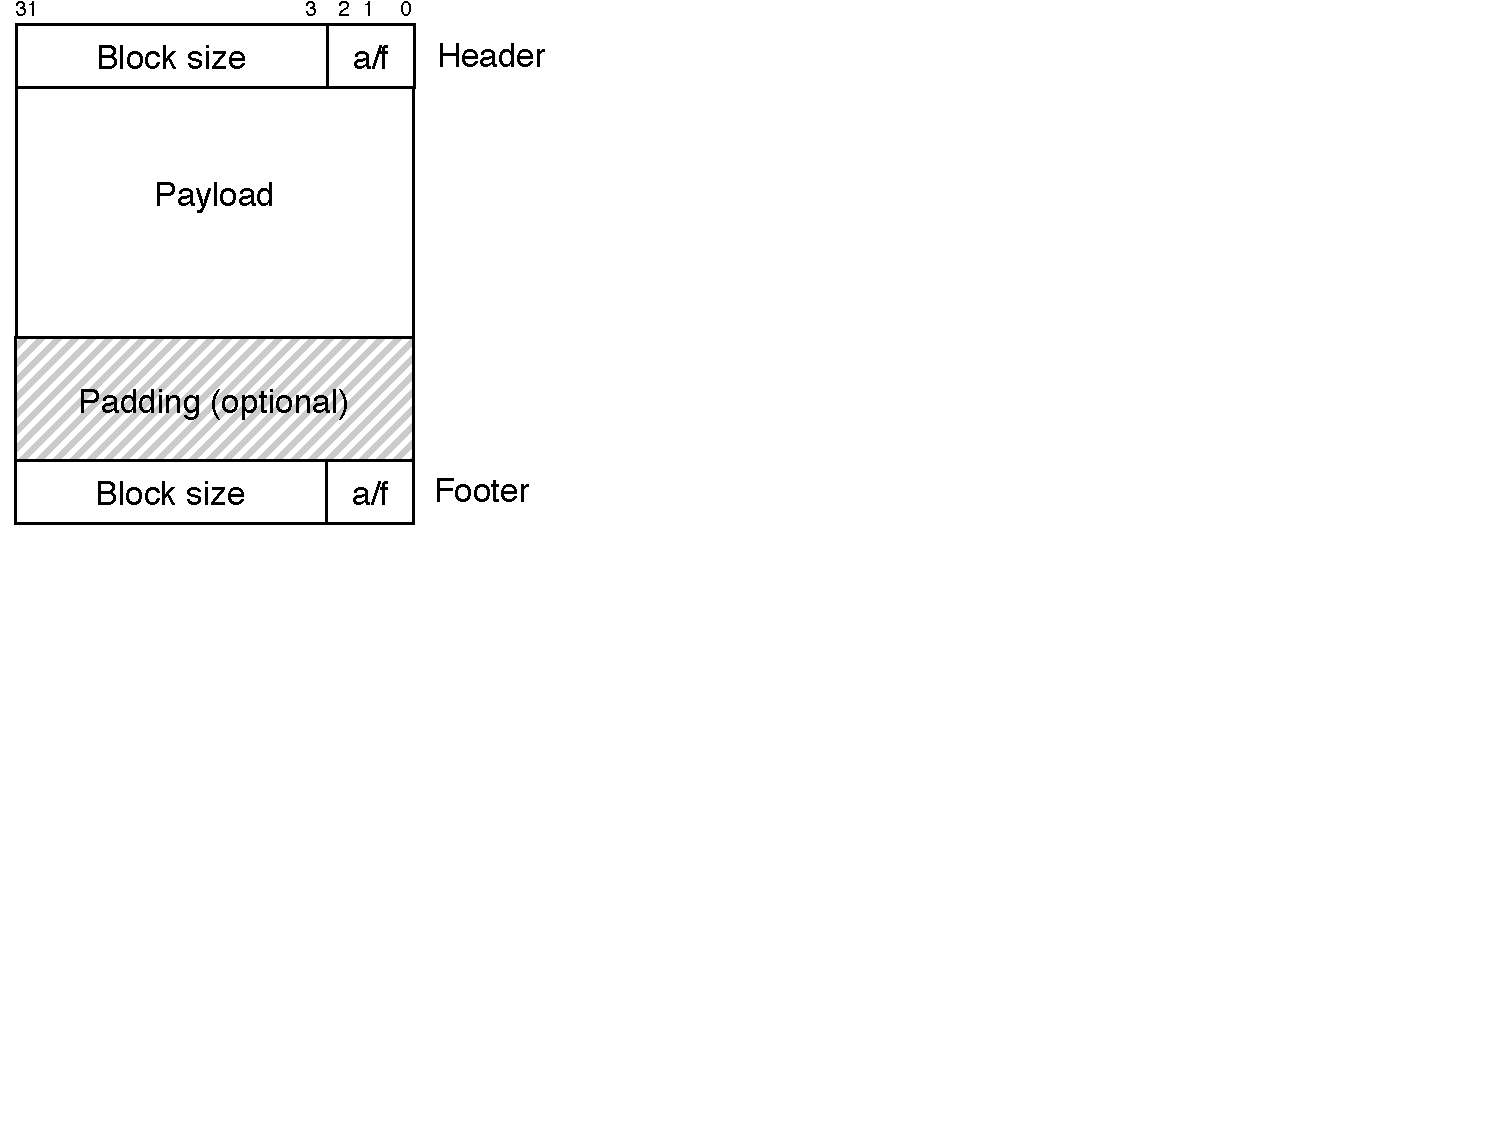
\includegraphics[width=0.3\textwidth]{linkedblocka.pdf}}
\ffigbox[0.35\textwidth]{\caption{Free block}}{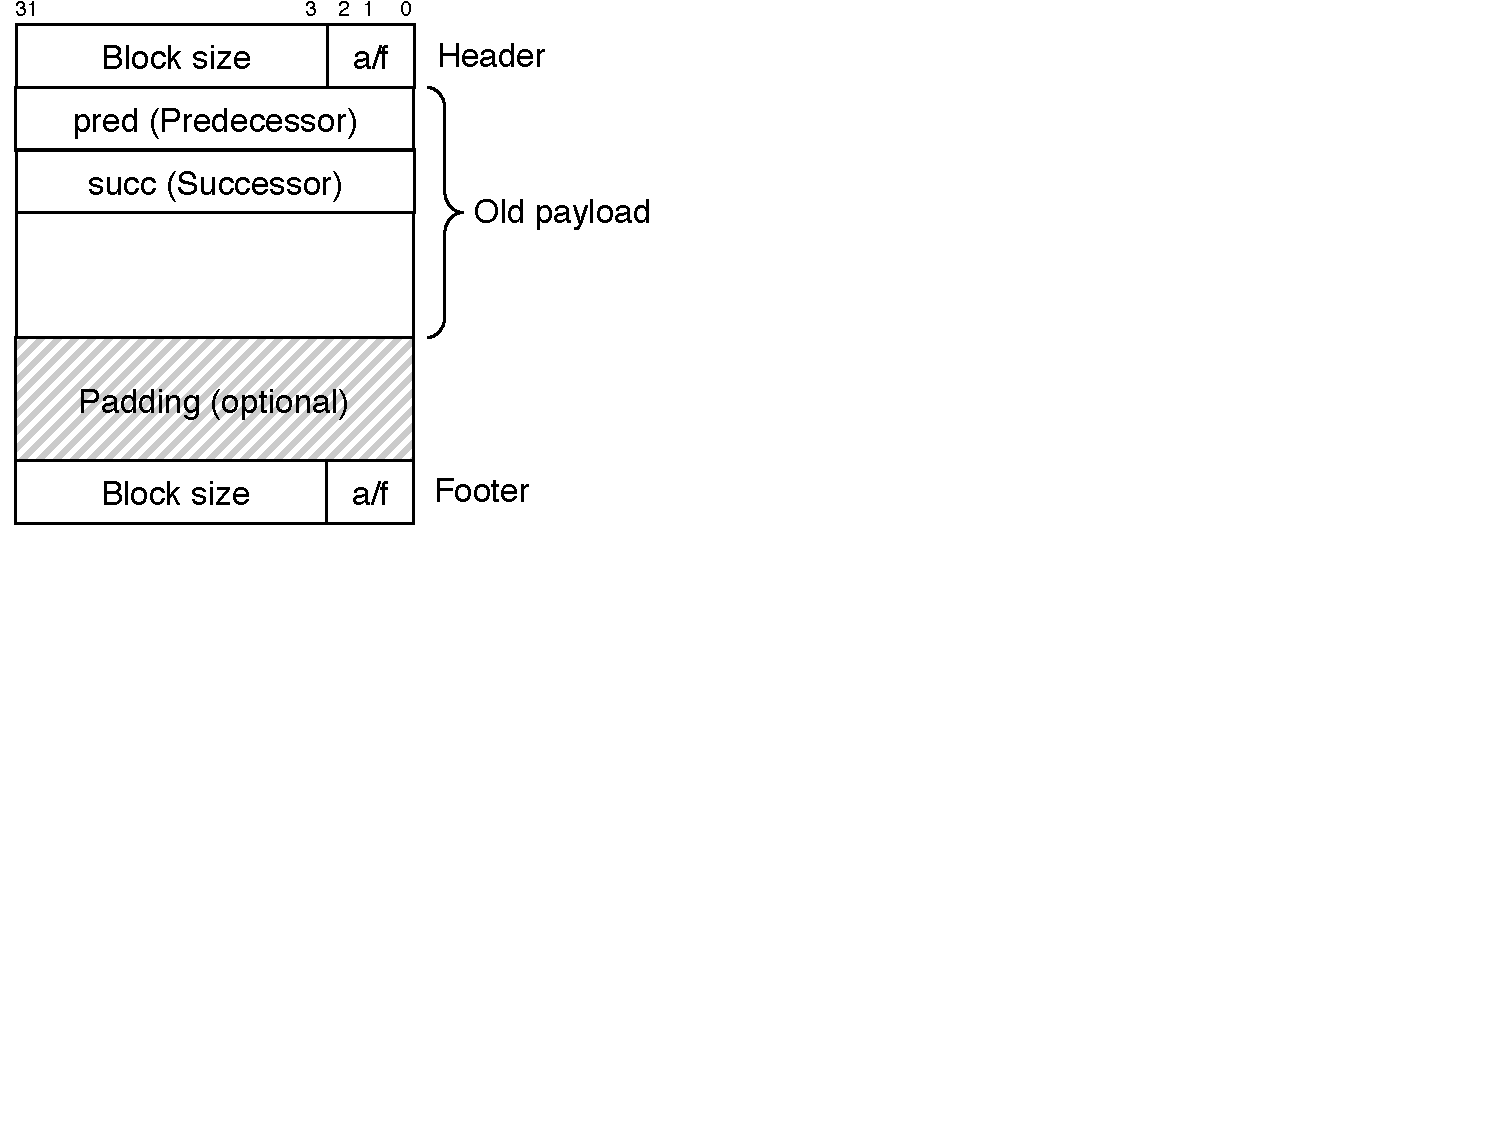
\includegraphics[width=0.35\textwidth]{linkedblockf.pdf}}
\end{subfloatrow}}
\caption{Format of heap blocks using doubly linked free lists}}
\end{figure}
Free time: depends on policy to order the blocks in the free list.
\begin{itemize}
	\item LIFO: inserting a newly freed block at the beginning of the list. Guarantees constant free of blocks.
	\item Maintains blocks in address order: linear free time, yet better memory utilization. 
\end{itemize}
\subsubsection{Segregated free lists}
Segregated storage: maintain multiple free lists to reduce allocation time. Partition the set of all possible block sizes into equivalence classes called size classes, e.g. by power of 2:
\[\{1\}, \{2\},\{3,4\},\{5,6,7,8\},\dots,\{1025-2048\},\{2049-4096\},\{4097-\infty\}\]
Or maybe assign small blocks to their own size classes, e.g. a size class for each of 1-1024. Each size class has its own free list. 
\subsubsection{Garbage collection}
Reachability graph: each node is an allocated memory block. An edge $p\rightarrow q$ means some position in p holds a pointer to some position in q. Root node of the graph: out-of-heap position holding pointers pointing to positions in the heap, e.g. registers, stack variables, global variables, etc. If there exists a path from any root node to a node p, then p is reachable. At anytime, unreachable nodes correspond to garbage that can no longer be used by the application, and thus should be reclaimed. The garbage collector maintains some representation of the reachability graph, frees unreachable nodes and returns them to the free list. Since C does not maintain any type information for memory locations, there is no obvious way to determine if a variable is a pointer, neither is there an obvious way to tell if it points to a position inside an allocated block. A garbage collector implemented for C has to be conservative: there are false positives when detecting reachable nodes.
\begin{figure}[ht]
\centering
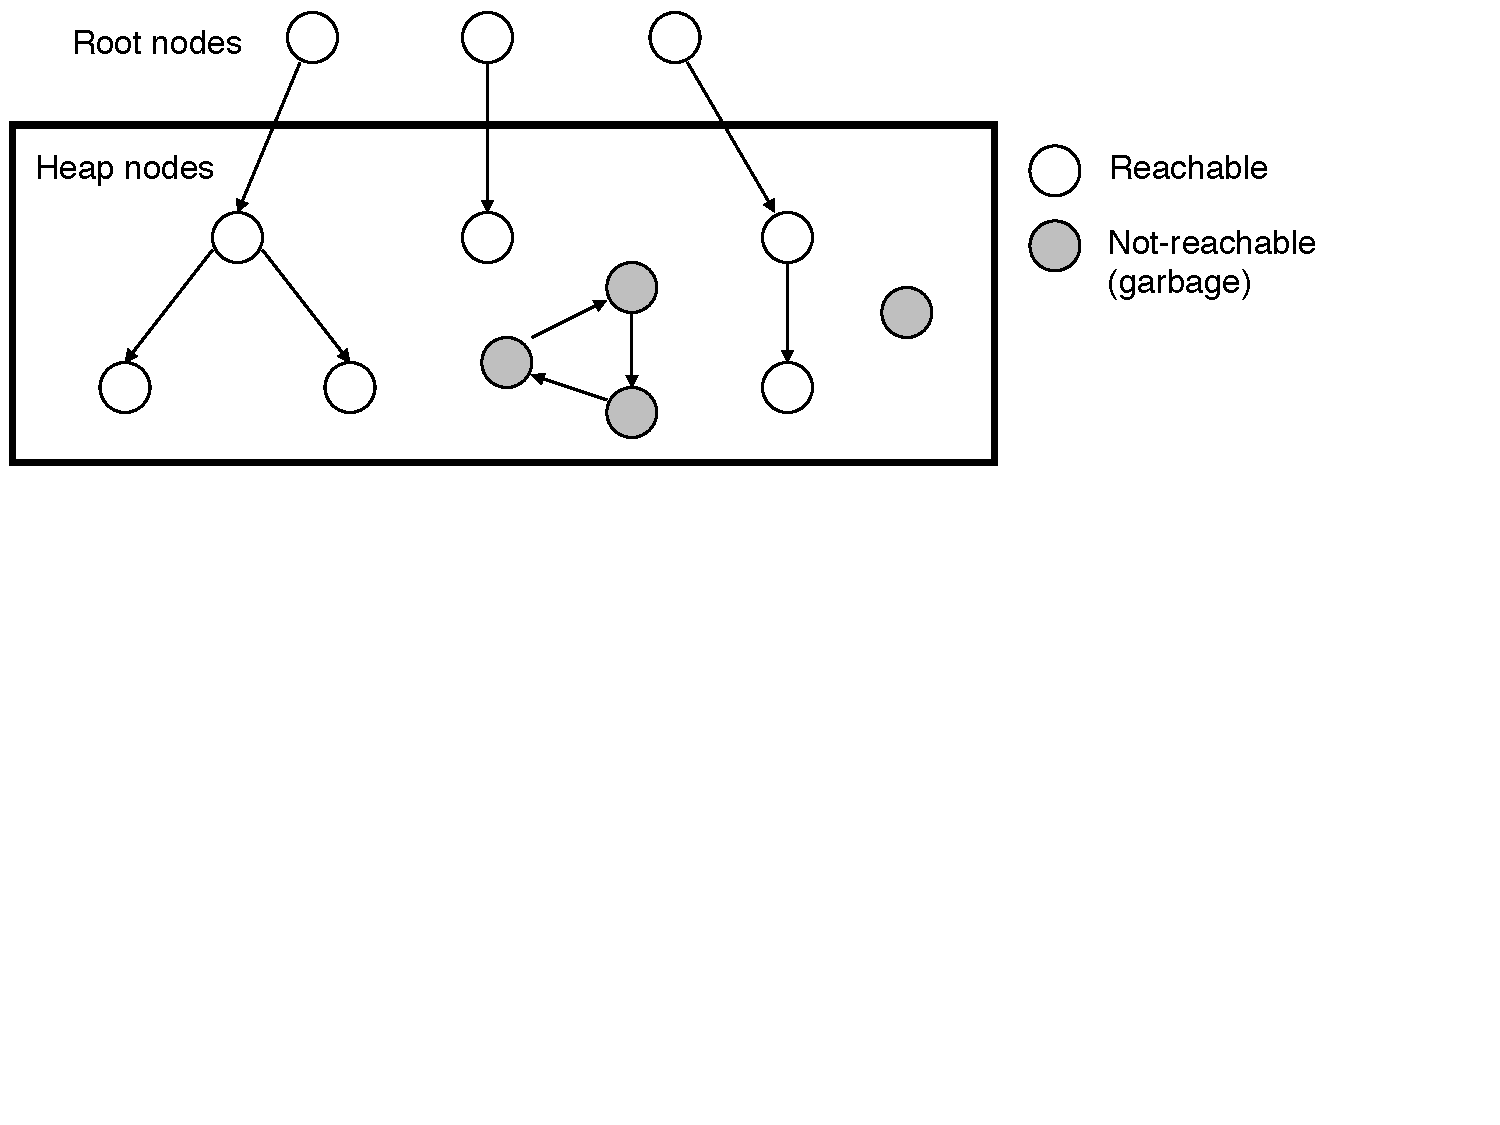
\includegraphics[width=\textwidth]{reach_graph.pdf}
\caption{Reachability graph}
\end{figure}
\ifx\PREAMBLE\undefined
\end{document}
\fi